\documentclass{article}

\usepackage[backend=biber,style=apa]{biblatex}
\addbibresource{bibliography.bib}

\usepackage[edges]{forest}
\usepackage{hyperref}

\author{Group 40}
\title{Design Document}

\begin{document}

\maketitle

\section{Abstract}

In this paper we will first introduce the \emph{non-obvious stakeholder} from the
Responsible Computer Science assignment, as it is credited for the focus on the `accessibility'
\emph{usability heuristic} from \textcite{Nielsen1994},
reviewed later in the Human-Computer Interaction assignment.

In chapter \hyperref[ethics]{2} we explore our choice for the \emph{visually impaired user} as the \emph{non-obvious stakeholder}
. In both chapters  \hyperref[ethics]{2} and  \hyperref[hci]{3}, we explore our choice for \emph{accessibility} as an
\emph{instrumental value} and  \emph{Nielsen heuristic} for the \emph{usability} analysis. \parencite{Nielsen1994}

    
\section{Responsible Computer Science Assignment:\\Responsible Design\label{ethics}}

To address the question ``In what way would our design process and final product change if we
also designed our product for one additional value of a ‘non-obvious’ stakeholder?'', we will discuss the stakeholders of the product, their values and their impact on the design process in the subsections that follow.

\subsection{Stakeholders\label{stakeholders}}

According to \textcite{Investopedia-stakeholder}'s definition of a stakeholder, direct stakeholders are individuals whose ``interest comes through a direct relationship,
such as employment, ownership, or investment'', whereas indirect stakeholders are individuals who
are not involved directly but still affected. We have therefore identified the role of our `Client' (also regarded in CSE1105 as CTA)
to be the actual `Sponsor' of the project, a direct stakeholder, as most of the development backlog is
catered towards his interests. Table \hyperref[stakeholdersTable]{1} shows the 9 product stakeholders divided into direct and indirect in concordance with
\textcite{Investopedia-stakeholder}.

\begin{table}
\centering
\begin{tabular}{||l c c ||} 
 \hline
 Stakeholder & Direct & Indirect \\
 \hline\hline
 Product developers & yes & no\\
 Student user & no & yes \\ 
 Staff user & no & yes \\
 \textbf{Visually impaired user} & no  & yes \\
 CTA/Sponsor & yes & no\\
 Rights-holder entity (TU Delft) & yes & no\\
 Third party infrastructure & no & yes  \\
 New customers (universities) & no & yes \\
 Cloud shared development environment & yes & no \\
 \hline
\end{tabular}
\caption{8 product stakeholders}
\label{stakeholdersTable}
\end{table}

\subsection{Non-obvious stakeholder: The visually impaired user\label{stakeholderMinority}}

To maximize the readability of the product for the widest range of users we have selected non-obvious stakeholder
to be the `visually impaired'. \textcite{Darroch2005} observed different preferences of font-sizes among age groups, and
\textcite{Hobbins2018} realizes the need for designing a GUI color scheme compatible with
colorblind people, who constitute 5{\%} of our Caucasian male population.
We have combined these two observations for the `visually impaired' stakeholder.

\subsection{Ethical values for the visually impaired \label{valuesMinority}}

\textcite{Zimmerman2019} acknowledges the use of the term `instrumental value' as a synonym of `extrinsic value' in his
analysis of intrinsic vs extrinsic values. He characterizes intrinsic values as
being some sort of moral, inherent good, and extrinsic values to derive their goodness from something else to which they are related.

Based on that definition, we presume the values listed below to be ethically relevant for the visually impaired.

\begin{enumerate}
    \item \textbf{Accessibility}: In accordance to the `interactionist' take on values in Value Sensitive Design \parencite{Friedman2013},
    we interpret accessibility as being an instrumental good or value to facilitate the intrinsic good of `equality'.
    \item \textbf{Equality}: Listed by \textcite{Frankena1973} as an intrinsic good and explicitly coined as ``just distribution of goods''.
    We believe that we should strive for good \emph{`usability'} \parencite{Nielsen1994} among all users.
    \item \textbf{Aesthetics}: Regarded by \textcite{Frankena1973} as `aesthetic experience', we find that optimizing the GUI for
    visually impaired users should not compromise the aesthetic experience of the average user nor the visually impaired themselves.
\end{enumerate}

\subsection{Accessibility\label{accessibility}}

`Accessibility' was introduced as an instrumental value for `equality' in section \hyperref[valuesMinority]{2.3} while `equality' regarded
the actual \emph{`usability'} of the product.

We refer to the term `usability' as one of the `usability heuristics' presented by \textcite{Nielsen1994} in the
`heuristic evaluation' design process discussed in chapter \hyperref[hci]{3}.

We have selected `accessibility' as the value to focus on both assignments as it overlaps in both fields, the academic ethics as
an instrumental value \parencite{Zimmerman2019} and as a usability heuristic \parencite{Nielsen1994} in Human-Computer Interaction.
We have also decided to focus on `accessibility' as it is a pragmatic approach to reach the 3 values simultaneously, since equality can
be achieved by providing an accessible yet aesthetic product.

The instrumental value of accessibility is covered by \textcite{Nielsen1994} as the `Flexibility and efficiency of use' heuristic,
which states that a product must allow for customization and efficiency of use. These requirements are covered in sections
\hyperref[stakeholderSupport]{2.5} (accommodating the design process for stakeholder needs), \hyperref[valueHierarchy]{2.6} (\emph{`value hierarchy'} analysis)
and \hyperref[stakeholderConflict]{2.7} (solving stakeholder values conflicts).

\subsection{Responsive design: learning about the visually impaired\label{stakeholderSupport}}

To learn more about the chosen stakeholder in the context of `accessibility', we have integrated an
`heuristic evaluation' at the beginning of the design process, immediately following the confirmation of the development backlog with the project `Sponsor' stakeholder.

\begin{quote}
``Heuristic evaluation is a usability engineering method for finding the usability problems in a user interface design so that
they can be attended to as part of an iterative design process.'' \parencite{Nielsen1994}
\end{quote}

In section \hyperref[experts]{3.2.1} we reveal that the type of experts we contacted were computer science students with
various degrees of expertise in the user experience design field. They were requested to fill-in the usability survey in \hyperref[survey]{4.1}.
%remember to send survey to Philipp (expert)

It is important to note that we have also sent the survey to a subset of the visually impaired, as we requested our fellow students
to send the usability survey to their older relatives, for which we prepared an A/B testing version of either the control or the  experiment ``wireframe'',
which were prototype designs of the product to test how different stakeholders react to the `accessibility' driven
design changes in the product. The other subset of the visually impaired, namely the colorblind, were difficult to collect in significant sizes, therefore
we've used the work of \textcite{Hobbins2018} from which we selected one of the recommended colorblind friendly color themes.

The complete evaluation and improvement process of the GUI design can be found in chapter \hyperref[hci]{3},
and the list of colorblind friendly color themes in section \hyperref[colors]{4.2}.

\subsection{Value Hierarchy\label{valueHierarchy}}

Figure \ref{tree} shows our implementation of the value hierarchy by \textcite{vandePoel2013} for the `accessibility' value.
The top layer or the ``root'' is `Accessibility', the value we've chosen to focus on. The second layer are the \emph{norms} that follow
from \emph{accessibility},  and the third layer or ``leafs'' are the \emph{design requirements} derived from their respective norms.

\begin{figure}
\centering
\begin{forest}
    forked edges,
    for tree={draw,align=center,edge={-latex}}
    [Accessibility
        [Natural interaction\\with the system
            [Clicks]
            [Undo]
        ]
        [Customisable\\interface
            [Color]
            [Text size]
        ]
        [Support for\\shortcuts
            [Mouse]
            [Keyboard]
            [GUI]
        ]
    ]
\end{forest}
\caption{Value Hierarchy \parencite{vandePoel2013} for \emph{accessibility}.}
\label{tree}
\end{figure}

Both the \emph{norms} and the \emph{design requirements} for `accessibility' have been adapted from \textcite{Nielsen1994} heuristic ``Flexibility and efficiency of use''.

\begin{itemize}
    \item Clicks: Make the graphical user interface (GUI) easy to use for the visually impaired by
    minimizing the number of clicks required to achieve a desired task. More formally: ``at most 2 clicks to execute a task''.
    \item Undo: Make actions reversible as the visually impaired are more prone to make errors.
    \item Color: By default use a colorblind friendly theme. Allow for further custom color themes.
    \item Text size: Allow for text size customization.
    \item Mouse: Allow for standard mouse shortcuts. This minimizes the user reliance on the GUI.
    \item Keyboard: Allow for keyboard shortcuts for the same reason.
    \item GUI: The GUI should provide standard `macro' functions such as `select all comments', `delete all comments', to minimize
    cognitive effort from using the GUI.
\end{itemize}

%macro: tick all questions and remove all

\subsection{Stakeholder conflicts\label{stakeholderConflict}}

\subsubsection{Tension between old and new values}

The addition of more features, in this case for the visually impaired, may contribute towards overloading the user interface
, similar to that of an old web browser. To assess whether the average user is actually affected by the
appearance of more buttons we've conducted an A/B testing survey with 2 product ``wireframes'',
one without the visually impaired features and another one with them.

The results were positive towards including the visually impaired features and these can be examined in section \ref{results}.

To resolve these tensions, the results of the surveys were thoughtfully taken into consideration and, as a result, the product has default background, colour and font size choices that were carefully selected to be colourblind friendly. The user is also provided with a 'Customize display' option present in the 'Settings' menu. This feature not only allows them to choose any background colour, size and colour font for the questions, but to also change the general background of the application to any image of their liking, provided they input a URL. 
\subsubsection{Design solutions}
%explicitly ask for "acceptance of" "inclusion" and "equality" of "GUI design" in the survey.
We have asked our survey respondents whether they accept the spending of resources on inclusive GUI design for minority users.
The survey results leaned towards inclusive GUI design, but in the hypothetical scenario where the average user
disapproves with inclusive GUI design, our project members will remain in accordance to our values,
compromising opinion of the major stakeholder. The project is open source, free of liabilities, and usability is according to free will. 

\subsubsection{Inclusive GUI survey}

The survey...

%word count: 1167

\section{HCI Assignment:\\GUI Evaluation \& Improvement\label{hci}}
%Max 2500 words long.

%Color palette justification. \parencite{Hobbins2018}
%font sized \textcite{Darroch2005}

\subsection{Introduction\label{introduction}}

In this chapter we explore our human-computer interaction analysis for the \textcite{Nielsen1994} heuristics:

\begin{itemize}
    \item Flexibility and efficiency of use: regarded in the previous chapter as `accessibility'.
    \item Visibility of system status: for the speed of the lecture and status of the questions (popularity and response).
    \item Aesthetic and minimalist design: comparison between `basic' and \emph{`visually impaired'} GUI features.
\end{itemize}

We performed the \emph{heuristic evaluation} before technical implementation of the application, by presenting our experiment participants with ``wireframes'',
(see Appendix in chapter \ref{appendix}) also known as prototype designs, of 2 potential design implementations, to A/B test the difference in
usability problems between a `basic' and a \emph{`visually impaired'} version of the product that would support for custom
color themes suitable for colorblind people and different font sizes for the graphical user interface.

\subsection{Methods\label{methods}}

\subsubsection{Experts\label{experts}}

In total 12 participants completed the survey, appended in section \ref{survey}, with 1 self-reported expert in the UX field,
2 with experience in the field and 9 novices in UX design.

Which according to the `number of evaluators' formula of \textcite{Nielsen1994}

$$f(i) = (1-(1-\lambda)^i)$$

with $f(i)$ as the \% of problems found, $\lambda$ as the \% found by a single evaluator and $i$ the number of evaluators, 
they should have found at least 98\% of the problems for the heuristics in the study. ($\lambda$ = .29, i = 12)

$$f(i) = (1-(1-.29)^{12})=.98359$$

The choice of lambda is mapped from \textcite{Nielsen1994} thumb rule where different levels of experts have different lambda
values: around .22, .45 and .60 for average, expert, master respectively.

We have therefore used the weighted average for the suggested values of lambda and the number of participants for each level of expertise:

$$\lambda = \frac{1}{12} \cdot 60 + \frac{2}{12} \cdot 45 + \frac{9}{12} \cdot 22 = 29$$

The participants consisted of a homogeneous demographic, all of whom reported to be in the Zoomer generation, in principle because it was demanded
that these were students taking this same course (CSE1105).

Regarding eye vision demographics, none of the participants were colorblind and only one sixth reported to need to increase the font size
when reading from electronic devices. The rest did not report to have vision problems.

Due to the nature of the participant requirements from the course, it was not possible to gather a statistically significant sample that represents all potential users of the application, namely TU Delft teaching staff and students.

\subsubsection{Procedure\label{procedure}}

Due to COVID-19, the heuristic evaluations had to be performed online. Consequently, we sent the survey in \ref{survey} to the experts
via a link to a \emph{Microsoft Forms} questionnaire, in which they were first prompted to fill in demographic information about
the generation they belong to, their expertise in the `user experience' design or related field, and their visual disabilities.

In the next sections of the survey, the respondents were introduced to the prototype design,
`basic' or a `visually impaired' wire-frame, depending on whether they were in the control group or in the experiment group,
as we also aimed to measure the difference in \emph{usability}.

Then for each of the the 3 heuristics introduced in section \ref{introduction}, namely ``Flexibility and efficiency of use'', ``Visibility of system status'' and
``Aesthetic and minimalist design'', we provided first a definition of the heuristic so that the respondents could exactly
now which aspects to focus on, and subsequently a picture of the wire-frame, which remained visible at all times during the survey.

After presenting the definition of the heuristic and the wire-frame, for each heuristic, the respondents were first asked to answer
the open questions about the problem description in a standardized way to maximize the precision of their answers \parencite{Nielsen1994}.
The brief problem description ought to include 2 aspects, first the context in which the problem occurred, and second its assumed cause.

Only after answering the open question, the respondents were shown in the next page of the survey a series of a 5 point Likert-scale
statements in which they had to agree or disagree with the extent to which certain usability problems applied to them for the
`flexibility and efficiency of use' and `visibility of system status' heuristics. For the `aesthetic and minimalist design' heuristic
the respondents were only asked to score the overall aesthetic experience.

All the questions asked in the survey can be found in the appendix in \ref{survey}.

\subsubsection{Measures (Data collection)}

To measure the \textbf{impact} of the usability problems we used the standardized z-scores from the 0-4 point scale questions
and to measure the \textbf{frequency} we counted how often they were mentioned in the open questions and turned
the frequencies into z-scores as well.

Although the data distribution was skewed to the left, we decided to implement z-scores to translate the position of the 0-4 point
scale questions, including the aesthetics 0-10 point scale question converted to a 0-4 point scale. This serves our interest to compare
the 2 different metrics and the z-scores allow for a fair comparison of scores on differently scaled variables,
namely impact and frequency, and also allows for a comparison of variables with different sample, mean, and standard deviation
\parencite{zscore}, such as the frequency metric retrieved
by the unassisted participant's ability to identify problems, and the Likert-scale questions regarding the impact of the problems
which were always collected regardless of whether the participants found the problem or not.

Finally, the score sign for the impact metric had to be reversed, as the questions originally used positive usability statements.

\subsection{Results\label{results}}

\subsubsection{Survey results\label{surveyresults}}

The participants spent 15 minutes on average to complete the survey, which is a reasonable amount given the format, in which they
only had to focus on a subset of the Nielsen usability heuristics, namely `accessibility', `visibility' and `aesthetics'.

The open questions for each of the usability heuristic have been interpreted and grouped
into the following problems:

\begin{itemize}
    \item Accessibility: Submit question does not feel natural - frequency: 2
    \begin{itemize}
        \item suggestion: (copy Facebook format and) place it lower on the screen - frequency: 2
        \item Map impact from:
        \begin{itemize}
            \item ``I could easily find out how to ask a question"
            \item ``I could easily understand the purpose of the application"
        \end{itemize}
    \end{itemize}
    \item Accessibility: Reading/Answering does not feel natural - frequency: 5
    \begin{itemize}
        \item suggestion: Increase the contrast color between question, response, and polls - frequency: 1
        \item suggestion: Increase the font size of the question area - frequency: 2 
        \item suggestion: avoid kahoot style buttons and place answer next to the button - frequency: 1
        \item suggestion: change green red contrast of NOT CORRECT / CORRECT (which are not colorblind friendly) to a softer palette and lowercase the words - frequency: 1
        \item Map impact from:
        \begin{itemize}
            \item ``I could easily find out how to ask a question"
            \item ``I could easily find out how to communicate to the lecturer about his/her speed"
        \end{itemize}
    \end{itemize}
    \item Accessibility: Lack of user control (unclear GUI menu) - frequency: 2
    \begin{itemize}
        \item suggestion: make clear how to leave the room - frequency: 1
        \item suggestion: make clear how to sort questions by which parameter - frequency: 1
        \item Map impact from:
        \begin{itemize}
            \item ``I could easily guess where to click to find out about the GUI customization options"
        \end{itemize}
    \end{itemize}
    \item Visibility: Unclear status of question - frequency: 2
    \begin{itemize}
        \item suggestion: make more explicit that a question has been answered - frequency: 1
        \item suggestion: make more explicit which questions belong to you - frequency: 1
        \item Map impact from:
        \begin{itemize}
            \item ``I could easily identify which questions were answered"
        \end{itemize}
    \end{itemize}
    \item Visibility: Unclear popularity of question - frequency: 1
    \begin{itemize}
        \item suggestion: make up-vote icon more explicit - frequency: 1
        \item Map impact from:
        \begin{itemize}
            \item ``I could easily identify the popularity of the questions"
            \item ``I could easily find out how to vote a question''
        \end{itemize}
    \end{itemize}
    \item Visibility: Speed of the lecture - frequency: 0
    \begin{itemize}
        \item Map impact from:
        \begin{itemize}
            \item ``I could easily identify the speed of the lecture"
        \end{itemize}
    \end{itemize}
    \item Visibility: Number of participants - frequency: 0
    \begin{itemize}
        \item Map impact from:
        \begin{itemize}
            \item ``I could easily identify the number of participants in the lecture"
        \end{itemize}
    \end{itemize}
    \item Aesthetics: Popularity icon - frequency: 2
    \begin{itemize}
        \item suggestion: Enlarge icon - frequency: 1
        \item suggestion: make up-vote icon more explicit - frequency: 1
        \item Map impact from:
        \begin{itemize}
            \item ``Overall aesthetics score"
        \end{itemize}
    \end{itemize}
    \item Aesthetics: Color contrast - frequency: 2
    \begin{itemize}
        \item suggestion: Questions should standout over participants/speed of lecture - frequency: 1
        \item suggestion: Use a background color in the questions section - frequency: 1
        \item Map impact from:
        \begin{itemize}
            \item ``Overall aesthetics score"
        \end{itemize}
    \end{itemize}
    \item Aesthetics: Style: 3
    \begin{itemize}
        \item quote: ``It looks too full, the design could be more simple" - frequency: 1
        \item quote: ``The aesthetic is quite a rudimentary one yet practical somehow" - frequency: 1
        \item quote: ``It looks more like a general site to ask questions" - frequency: 1
        \item Map impact from:
        \begin{itemize}
            \item ``Overall aesthetics score"
        \end{itemize}
    \end{itemize}
    
\end{itemize}     

``Map impact" refers to the Likert-scale questions for usability problems asked after answering the open questions.
In the case of the aesthetic heuristics, ``map impact" refers to the 0-10 point aesthetic score.

\subsubsection{z-scores and Prioritizing  Severity Matrix\label{severityanalysis}}

In total 120 scores were retrieved (12 per Likert-scale question), with $\mu = 3.0366\dots$, $\sigma=1.013897869$ and $Z=(x-\mu)/\sigma$ where
Z stands for the standardized value for a respondent's answer x.

The final standardized scores for each of the 10 usability problems described in \ref{surveyresults} were calculated by taking the
average of all participants responses of the mapped questions to the usability problem.

The frequencies were also standardized for each of the 10 usability problems, with $\mu = 1.9$, and $\sigma=1.374772708$.

This resulted in the prioritizing severity presented in figure \ref{severitymatrix}.

\begin{figure}
    \centering
    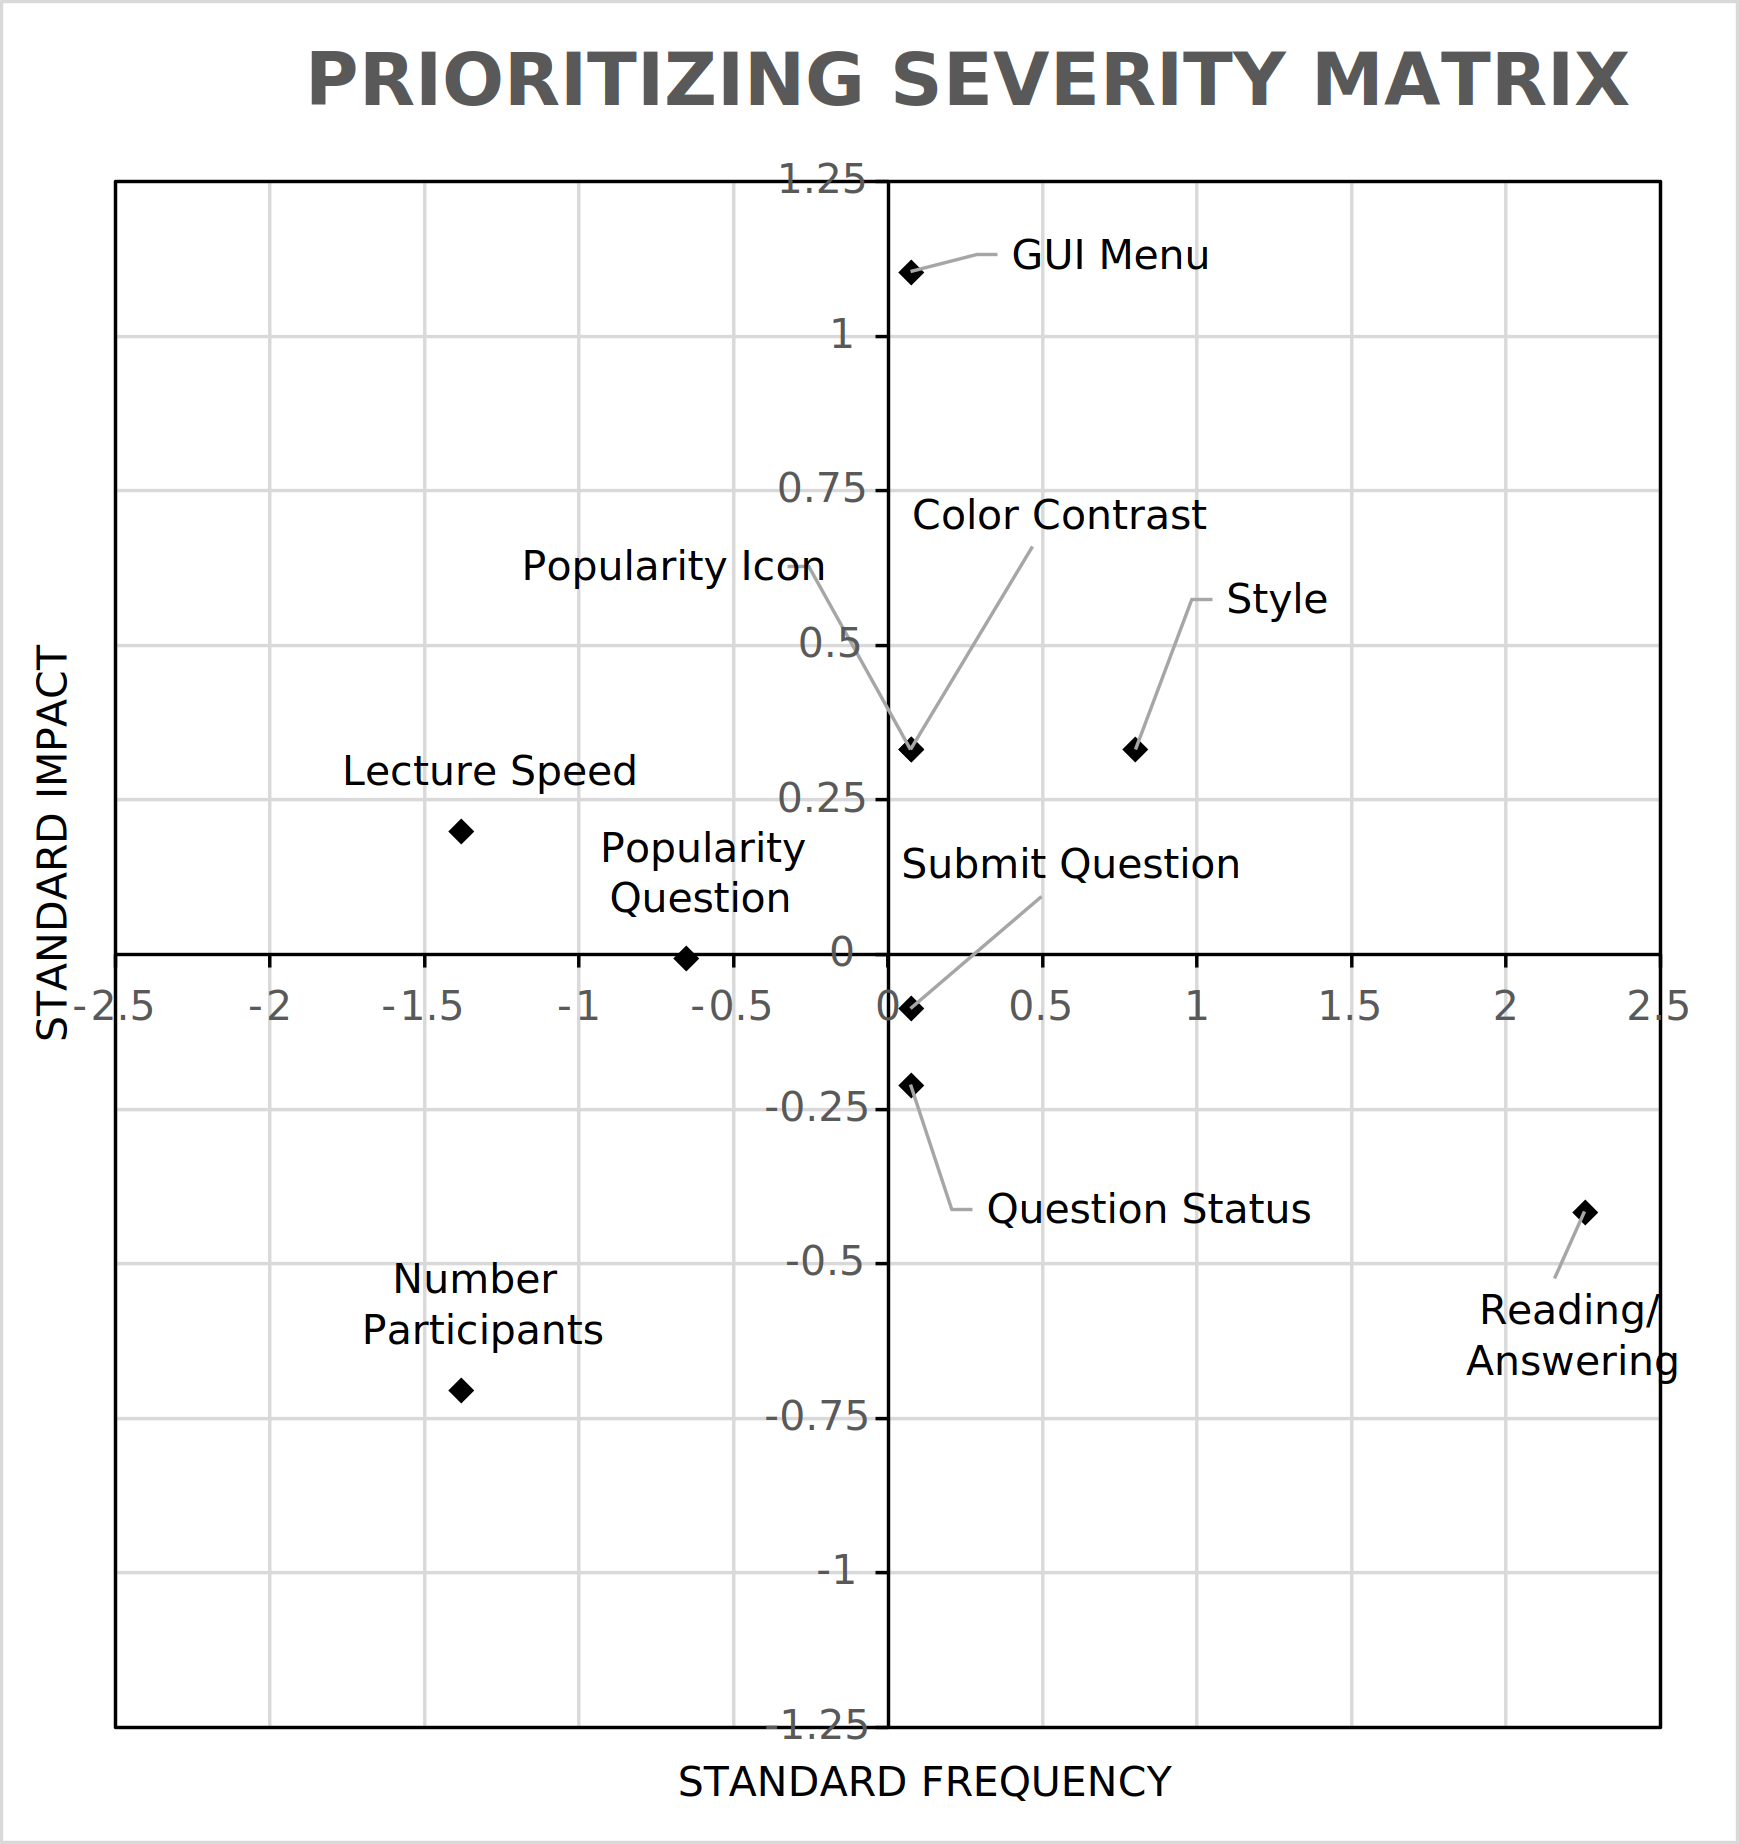
\includegraphics[width=\textwidth]{matrix.png}
    \caption{Prioritizing Severity Matrix}
    \label{severitymatrix}
\end{figure}

The final priority of the problem is calculated by taking the average of the standard frequency and the standard impact, 
which the table \ref{scores} represents as percentages for better comprehensibility. Furthermore, these priority scores were placed in Severity bins
with the following intervals:

\begin{itemize}
    \item Very low: Less than -60\%
    \item Low: [-60\%,-20\%)
    \item Medium: [-20\%,20\%]
    \item High: (20\%, 60\%]
    \item Very High: More than 60\%
\end{itemize}

\begin{table}[ht]
    \centering
    \begin{tabular}{||l c c c c ||} 
     \hline
     Problem & Std. frequency & Std. impact & Priority & Severity \\
     \hline\hline
     Reading/Answering & 2.2549 & -0.4159 & 92\% & Very High\\
     GUI Menu & 0.0727 & 1.1046 & 59\% & High\\
     Style & 0.8001 & 0.3321 & 57\% & High\\
     Popularity Icon & 0.0727 & 0.3321 & 20\% & Medium\\
     Color Contrast & 0.0727 & 0.3321 & 20\% & Medium\\
     Submit Question & 0.0727 & -0.0871 & -1\% & Medium\\
     Question Status & 0.0727 & -0.2104 & -7\% & Medium\\
     Popularity Question & -0.6547 & -0.0049 & -33\% & Low\\
     Lecture Speed & -1.3820 & 0.2005 & -59\% & Low\\
     Number Participants & -1.3820 & -0.7036 & -104\% & Very Low\\
     \hline
    \end{tabular}
    \caption{Prioritizing Severity}
    \label{scores}
    \end{table}

The problems refer more explicitly to:

\begin{itemize}
    \item Reading/Answering: ``Reading/Answering does not feel natural'' (Accessibility)
    \item GUI Menu: ``Lack of user control (unclear GUI menu)'' (Accessibility)
    \item Style: ``Layout style'' (Aesthetics)
    \item Popularity Icon: ``popularity icon'' (Aesthetics)
    \item Color Contrast: ``Background color/contrast between sections'' (Aesthetics)
    \item Submit Question:``Submit question does not feel natural'' (Accessibility)
    \item Question Status: ``Unclear status of question'' (Visibility of system status)
    \item Popularity Question: ``Unclear popularity of question'' (Visibility of system status)
    \item Lecture Speed: ``Lecture speed poll'' (Visibility of system status) 
    \item Number Participants: ``Number of participants'' (Visibility of system status)
\end{itemize}


\subsubsection{A/B Test\label{abtest}}

The survey participants were split into a control group and a test group, in which we provided the test group
with a slightly different wire-frame, to test the usability and aesthetics of the buttons for the the visually impaired features.

Figure \ref{ABGui} shows the difference between wire-frame A and wire-frame B.

\begin{figure}[ht]
    \centering
    \includegraphics[width=\textwidth]{wireframe_AB.png}
    \caption{A/B Test for visually impaired features}
    \label{ABGui}
\end{figure}

Although we were unable to collect a statistically significant sample, we successfully conducted the A/B experiment as it provides a structure to
collect user insights in support or against a potential version of the product. \parencite{Young2014}

From the survey results we received complaints that the design seemed ``too full", due to the ``many functionalities", and that it could be made simpler (\#8. Aesthetic and minimalist design)

One of the respondents mentioned:

\begin{quotation}
\emph{``...the customization menu is hard to see and also to operate.
I'm assuming a drop-down/popup menu would fit the cause better."}
\end{quotation}

Furthermore, if we account for outliers, we have learned that wire-frame B is not only preferred in terms of usability, but also aesthetically,
with 0-10 aesthetic scores of 7 and 7.4 respectively. The outlier low aesthetic score for wire-frame B did not regard issues related
to the A/B test feature, it is therefore statistically justified to disregard it. 

\subsection{Final design - usability heuristics correlation\label{usabilityheuristics}}

\subsubsection{Visibility of system status\label{1stheuristic}}
"The system should keep users informed about what is going on, with appropriate feedback in good time."
(\textcite{Nielsen1994})
Aspects of the design corresponding to this heuristic:

\begin{itemize}
    \item Questions are updated in real time, with relevant information about
    \begin{itemize}
        \item Number of votes
        \item Status of the question (answered or not)
        \item Reply (did the question receive a reply from moderators)
    \end{itemize}
    \item The list of users which is updated automatically 
    \item A drop-down containing the already answered questions is present, to encourage the user to avoid repetitive questions
    \item The speed poll which is open throughout the lecture through which the lecturer can retrieve valuable opinions from students regarding the lecture's speed
    \item The ability to create live polls, with multiple options, in order to check the students' level of understanding of the information presented in the lecture
    \item The action of up-voting a question can lead to immediate changes in the questions' order presented to the student and moderator
    \item The ability to see (live) if a reply to a question is being typed, thus avoiding collisions between moderators (multiple moderators answering the same question)
    \item Editing a question yields immediate visual results without affecting any other attribute of the question
\end{itemize}


\subsubsection{Match between system and the real world\label{2ndheuristic}}
"The system should speak the users language, with words, phrases, and concepts familiar at the user (not technical terms)." (\textcite{Nielsen1994})
Aspects of the design corresponding to this heuristic:
\begin{itemize}
    \item There is an emphasis put on using less words and more interactive user interface elements, colors  
    \item The vocabulary employed is one of day-to-day basis, making it friendly to people who have less technology skills
    \item The words are written in a modern font having a size that can be adjustable, suitable to the user's needs
    \item Technical terms are avoided, with exception of terms like "logs" in the feature "export logs". This feature however has a "small target audience", being destined only for the technical moderators, not for the average user or for the lecturer
\end{itemize}

\subsubsection{User control and freedom\label{3rdheuristic}}
"System functions may be chosen by the user by mistake: they need a clearly marked 'emergency exit' without having to go through an extended dialogue." (\textcite{Nielsen1994})
Aspects of the design corresponding to this heuristic:
\begin{itemize}
\item 'Cancel' button to cancel the creation of a new lecture on the popup from clicking 'Start a new lecture directly' on the Home screen
\item 'Disable rate limit' option in the 'Settings' menu on the Moderator screen to undo enabling the rate limit
\item 'Cancel' button to cancel the creation of a new lecture on the Schedule screen
\item 'Back' button to return to the Home screen available on the Help page
\item 'Cancel' button to cancel banning a user when clicking the 'Ban user' option in the 'Settings' menu on the Moderator screen
\item 'Discard changes' button to discard the changes done to the background colour, size and colour font when clicking 'Customize display' option in the 'Settings' menu on the Moderator and Student screens
\item 'Cancel' button to cancel exporting the questions in the popup from clicking 'Export Questions' option in the 'Settings' menu on the Moderator screen
\item 'Cancel' button to cancel downloading the log in the popup from clicking 'Download log' option in the 'Settings' menu on the Moderator screen
\end{itemize}

\subsubsection{Consistency and standards\label{4thheuristic}}
"Users should not have to wonder whether different words, situations or actions mean the same thing." (\textcite{Nielsen1994})
Aspects of the design corresponding to this heuristic:
\begin{itemize}
\item The application use day-to-day vocabulary for all of the functionality features. This caters especially well to students as many terms we use are common to applications used already by students. 
\item The application does not use technical terms to describe functionality. 
\item The buttons, such as Vote and Mark as Answered, have an immediate response, such as changing color. This allows the user to distinguish the immediate visual result. 
\end{itemize}


\subsubsection{Error prevention\label{5thheuristic}}
"Even better than a good error message is a careful design which presents a problem from occurring in the first place." (\textcite{Nielsen1994})
Aspects of the design corresponding to this heuristic:
\begin{itemize}
    \item Design that is not prone to errors; the moderator and student screens are made in a way that they don't allow the user to make app-breaking mistakes
    \item The input is sanitized, doesn't allow for malicious interference with the database that can halt a live lecture
    \item Each button has been designed to be visible and clickable only in conditions in which clicking doesn't result in unusual or unauthorized activity (a user can edit or delete only his own questions, while a moderator can do so without any restrictions)
    \item The options in the settings drop-down:
        \begin{itemize}
            \item Unusual behaviour has no effect on the lecture (clicking start lecture twice has no effect)
            \item Clicking export questions or export logs pauses the application - not allowing the user to accidentally cause errors
        \end{itemize}
    \item The only errors a user can encounter occur in the join a lecture / create a lecture main screen (joining a lecture with a misspelled link - in which case the user receives a helpful pop-up alerting him about his mistake)
\end{itemize}
\subsubsection{Recognition rather than recall\label{6thheuristic}}
"Try to make objects, actions and options visible. The user should not have to mentally hold information and transfer it to another part of the interface. Instructions for using the system should be visible or easily retrievable whenever appropriate." (\textcite{Nielsen1994})
Aspects of the design corresponding to this heuristic:
\begin{itemize}
\item the Moderator and Student joining links visible on the Moderator screen at all times
\item the Pace of the lecture poll visible on the Moderator and Student screens at all times
\item all buttons ('Edit', 'Delete', 'Hide', 'Reply', 'Answered', 'Vote'/'Votes') which provide interaction with the questions on the Moderator and Student screens visible at all times
\end{itemize}

\subsubsection{Flexibility and efficiency of use\label{7thheuristic}}
"Accelerators (such as function keys or macros) and senior buyer of the novice user may often speed up the interaction of for the expert user. Thus the system that can cater to both inexperienced and experienced users." (\textcite{Nielsen1994})
Aspects of the design corresponding to this heuristic:
\begin{itemize}
\item There is a customisation feature in the application. The user can choose the text-size and the background picture. In this way, the application can easily be tailored for users of different expertise levels. 
\end{itemize}

\subsubsection{Aesthetic and minimalist design\label{8thheuristic}}
"Dialogues or other interface items should not contain information that is irrelevant or rarely needed. All information on the screen competes with relevant units of information, diminishing at their relative visibility." (\textcite{Nielsen1994})
Aspects of the design corresponding to this heuristic:
\begin{itemize}
\item "Settings Button" encapsulates many features such as banning users, receiving a file of questions asked during the lecture, etc. This provides a simple interface for the users, while maintaining all functionality. 
\end{itemize}

\subsubsection{Help users recognize, diagnose, and recover from errors\label{9thheuristic}}
"Helping users to recognise, diagnose and recover from errors. Error messages should be clearly expressed in plain language, precisely indicate the problem, and constructively suggest a solution." (\textcite{Nielsen1994})
Aspects of the design corresponding to this heuristic:
\begin{itemize}
\item Our final application has a "Help Page" at the start of the application in order to facilitate the user's understanding of the application. This informs the user of potential errors or usability problems. 
\end{itemize}

\subsubsection{Help and documentation\label{10thheuristic}}
"Although the system should be able to be used without documentation, it may be necessary to provide help of some form. This information should be easy to search, focused on it the user's ongoing task (context sensitive), list the steps to be carried out, and be brief and to the point." (\textcite{Nielsen1994})
Aspects of the design corresponding to this heuristic:
\begin{itemize}
\item 'Help' button on the Home Screen which opens a popup informing the user on the purpose of the application and how to use it from a student or moderator point of view
\end{itemize}

\subsection{Conclusion and Improvements\label{conclusion}}

From the severity analysis in section \ref{severityanalysis} we have learned that the poor readability and answering of the questions
constitutes the largest severity problem, followed by the unclear GUI menu and the aesthetic layout of the application. Other concerns
pointed towards the question popularity visibility, the submit question accessibility and the question status visibility.

The popularity of the question visibility, the lecture speed poll visibility and the number of participants visibility did not
raise concerns.

We have translated the problems with a positive sign severity, namely Reading/Answering, GUI Menu, Style, Popularity Icon,
and Color Contrast, into the following backlog items, ordered by the priority from table \ref{scores}:

\begin{itemize}
    \item As a user, I want to see a clear button to leave/stop the lecture. (\#3. User control and freedom)
    \item As a user, I want to see explicit buttons for each type of sorting available.(\#3. User control and freedom)
    \item As a user, I want to experience a minimalist app design that feels like an online lecture-driven application. (\#8. Aesthetic and minimalist design)
    \item As a user, I want to see a large, recognizable (up arrow) upvote icon to upvote the questions. (\#3. User control and freedom)
    \item As a user, I want to easily distinguish between the questions, answers, polls and member sections by relying on
    different background colors. (\#8. Aesthetic and minimalist design)
\end{itemize}

As observed in the A/B Test in section \ref{abtest}, wireframe B was preferred. Therefore we have implemented the improvements
suggested by the survey results on wireframe B. Figure \ref{beforeafter} shows the before and after the survey wireframes.

We believe that the survey allowed the wireframe to be develop towards an improved GUI, as it now addresses all the usability problems whose severity
was High, Very High and the Mediums that had a positive priority score.

\subsubsection{Additional Remarks about Implementation\label{Implementation comments}}
While implementing the design choices and functionalities gathered through this research, we conducted some changes to comply with each user's needs.

The original color-blind theme of the application proved not to be as appealing for the client and other users as originally conducted from the survey. To make sure the application stays accessible and appealing for all users, we decided to change the application to make it possible for all kind of users to change the appearance of the application and allow them to change the following things:
\begin{itemize}
\item Each session starts with a common view that makes use of a simplistic modern design 
\item The standard view for the moderators has a different background than that of a public user. This way it is possible for a moderator to notice whether he has started his session correctly (Appendix 4.3.2).  
\item Each user can change the background for a session to any image of his or her choosing.
\item Each user can change the color of the text for a session.
\item Each user can increase/decrease the font size to accompany his own needs.
\end{itemize}
We also made some changes to the general non-customizable parts of the view.
The changes mostly increase the simplicity of the design.
Titled panes on the right side of the view (Appendix 4.3.2) are not expanded by default to keep the view less crowded.
The buttons that a user can use that are non-question related are summed up in a "settings" list and only shown when a user
clicks on the settings icon (Appendix 4.3.2).The initial design and the final design can be found next to each other
in Appendix 4.3.

Not only did we make changes in out initial design, but we also implemented some features that were described by the client
in slightly a different way.
We reached the conclusion that banning users based on IP Addresses would not most suitable for the application,
since there are many situations in which multiple students share the same internet connection and therefore IP Address,
which could mean that innocent users could be banned.
An example would be students in shared housing or at the university library; if one user is disrupting the lecture,
all users would be removed had banning been by IP address. Banning by User-Id makes it so that only individual disruptive
users are removed from the lecture.

The objective of the application is to provide an improved online communication tool between a large number of students and a lecturer. This communication occurs through questions about the lecture, and thus online lectures are currently suffering from problems such as, but not limited to:
\begin{itemize}
\item Chats are spammed with multiple repetitive questions
\item Lots of relevant questions are left unseen
\item Chats are usually filled with non-related commentaries
\item The lecturer answers outdated questions
\end{itemize}

We reached the conclusion that it is not enough for our application to let users ask questions to the lecturer, but it's mandatory to come up with a way in which the most relevant and sought questions are immediately visible to the lecturer, who usually has limited time to answer questions.
This can be achieved through proper sorting methods, and we decided to implement three of them:
\begin{itemize}
    \item TOP: Sorting questions by their number of upvotes, not taking into account time, thus the lecturer being able to see which questions are the most popular
    \item NEW: Sorting questions by the moment of time in which they were asked, not taking into account the number of votes, thus the lecturer is able to see only the newest and freshest questions
    \item HOT: Sorting questions by a formula that takes into account not only the number of upvotes, but the time too, thus increasing the level of interactivity in the lecture, since the lecturer can see the popular questions that are the most related to what he's teaching at a certain moment in time
\end{itemize}

\pagebreak
\section{Appendix\label{appendix}}
\subsection{HCI SURVEY\label{survey}}

Survey screenshots version B

\subsection{Colorblind friendly palettes\label{colors}}

According to \textcite{Hobbins2018}, these are the color combinations compatible with colorblind users:

\begin{itemize}
\item Red and blue
\item Red and purple
\item Orange and blue
\item Orange and purple
\item Brown and blue
\item Brown and purple
\item Yellow and blue
\item Yellow and purple
\item Yellow and gray
\item Gray and blue
\end{itemize}
\subsection{Final Design}
\begin{center}
    \label{beforeafter}
    \includegraphics[width=0.95\textwidth]{initial_design.JPG}
    Before (light theme and full opacity)
    \vfill
    \includegraphics[width=0.95\textwidth]{moderator_screen.JPG}
    After (customizable background image and transparent sections)
    \clearpage
    \label{studentmoderator}
    \includegraphics[width=0.95\textwidth]{student_screen.JPG}
    Default student screen (sea)
    \vfill
    \includegraphics[width=0.95\textwidth]{moderator_screen.JPG}
    Default moderator screen (mountain)
    \clearpage
    \label{settings}
    \includegraphics[width=0.5\textwidth]{pane_and_settings.JPG}
    \\Settings (minimalistic gear button and expandible panes)
    \clearpage
\end{center}
\printbibliography

\end{document}
